\documentclass[journal]{IEEEtran}
% Report 1 (Labs 1-4), CS605 Artificial Intelligence, IIIT Vadodara, Autumn 2026-27.
% Written for the IEEE Transactions on Systems, Man, and Cybernetics: Systems LaTeX
% template (IEEEtran, journal mode). To use the course template, paste the body of
% this file into it and keep refs.bib and figures/ alongside.
\usepackage{amsmath,amssymb,amsfonts}
\usepackage{graphicx}
\usepackage{booktabs}
\usepackage{multirow}
\usepackage{algorithm}
\usepackage{algpseudocode}
\usepackage{cite}
\usepackage{url}
\usepackage{xcolor}
\usepackage[hidelinks]{hyperref}
\graphicspath{{figures/}}
\newcommand{\st}[1]{\texttt{#1}}

\begin{document}

\title{State-Space Search, Heuristics and Randomised Local Search:\\ A Tutorial Through Four Laboratory Problems}

\author{[Student Name 1, Roll No.],~[Student Name 2, Roll No.],~[Student Name 3, Roll No.],~[Student Name 4, Roll No.]%
\thanks{CS605 Artificial Intelligence, Lab Report 1 (Labs 1--4), Group [XX], IIIT Vadodara, Autumn 2026--27. Instructor: Pratik Shah. Code: [group Git repository URL].}}

\markboth{CS605 Artificial Intelligence --- Lab Report 1}{Group [XX]}

\maketitle

\begin{abstract}
This report works through the first four CS605 laboratory problems as a tutorial on problem
formulation and search. We model the Missionaries-and-Cannibals and Rabbit-Leap puzzles as
state-space search problems and solve them with breadth-first (BFS) and depth-first search
(DFS) built on a single reusable graph-search agent; a counting argument shows why both
return the optimal 15-move Rabbit-Leap solution. We then cast plagiarism detection as a
shortest-path problem over partial sentence alignments and solve it with A$^*$ using
Levenshtein costs and three admissible heuristics, which halve the number of expanded nodes
relative to uniform-cost search. For uniform random 3-SAT we compare Hill-Climbing, Beam
Search (widths 3 and 4) and Variable Neighbourhood Descent with two heuristics in terms of
success rate and penetrance on 180 instances around the satisfiability phase transition.
Finally, we solve the scrambled-Lena jigsaw ($16! \approx 2\times10^{13}$ states) with
simulated annealing, show how the choice of energy and move set decides whether the
annealer finds the true image, and, as in-lab and challenge problems, plan an optimal
20-city tour of Rajasthan and generate a Raag Bhairav melody.
\end{abstract}

\begin{IEEEkeywords}
State-space search, BFS, DFS, A$^*$, admissible heuristic, Levenshtein distance, $k$-SAT,
hill climbing, beam search, variable neighbourhood descent, penetrance, simulated annealing,
jigsaw puzzle, travelling salesman problem.
\end{IEEEkeywords}

%=====================================================================================
\section{Introduction}
%=====================================================================================
\IEEEPARstart{A}{n} intelligent agent that solves a problem by search needs two things: a
\emph{formulation} that turns the informal task into states, actions, a transition model, a
goal test and a cost, and an \emph{algorithm} that explores the resulting graph
\cite{aima4}. The four labs in this report vary one of these at a time. Labs~1 and 2 keep the
algorithm family fixed (systematic graph search) and change the formulation, from toy puzzles
to text alignment. Labs~3 and 4 keep complete-state formulations but replace systematic search
by local and randomised search, because the state spaces ($2^n$ assignments, $16!$
permutations) are too large to enumerate.

All code is in Python; one graph-search agent (Section~\ref{sec:agent}) is shared by Labs~1
and 2. Every number in this report is produced by the scripts in the accompanying
repository, with fixed random seeds.

%=====================================================================================
\section{A Reusable Graph-Search Agent}\label{sec:agent}
%=====================================================================================
A problem object exposes the initial state, a goal test and a successor function returning
$(\text{action}, s', c(s,a,s'))$ triples. The agent (Algorithm~\ref{alg:graph}) keeps a
\emph{frontier} of nodes waiting to be expanded and a hash table \emph{reached} of states
already generated, so that every state is expanded at most once. A node stores its state,
its parent pointer, the action that produced it, the path cost $g$ and its depth; following
parent pointers from the goal back to the root reconstructs the solution path.

\begin{algorithm}[t]
\caption{Graph search with a pluggable frontier}\label{alg:graph}
\begin{algorithmic}[1]
\Function{GraphSearch}{problem, frontier}
  \State $n_0 \gets$ \Call{Node}{problem.initial}; frontier.push($n_0$)
  \State reached $\gets \{n_0.\text{state}: n_0\}$ \Comment{hash table}
  \While{frontier not empty}
    \State $n \gets$ frontier.pop()
    \If{problem.\Call{IsGoal}{$n$.state}} \Return \Call{Path}{$n$} \EndIf
    \For{$(a, s', c)$ \textbf{in} problem.\Call{Successors}{$n$.state}}
      \State $n' \gets$ \Call{Node}{$s'$, parent $=n$, $a$, $g = n.g + c$}
      \If{$s' \notin$ reached \textbf{or} $n'.g <$ reached[$s'$]$.g$}
        \State reached[$s'$] $\gets n'$; frontier.push($n'$)
      \EndIf
    \EndFor
  \EndWhile
  \State \Return failure
\EndFunction
\end{algorithmic}
\end{algorithm}

The frontier discipline selects the algorithm: a FIFO queue gives BFS (with the goal test
moved to generation time, which is safe for unit costs), a LIFO stack gives DFS, and a
priority queue ordered by $f(n)$ gives uniform-cost search ($f=g$), greedy best-first
($f=h$) or A$^*$ ($f=g+h$) \cite{aima4}. A stale-entry check (``is this still the best node
for its state?'') replaces the decrease-key operation that binary heaps lack.

%=====================================================================================
\section{Lab 1: Uninformed Search on Two River-Crossing Puzzles}
%=====================================================================================
\subsection{Missionaries and Cannibals: formulation}
Amarel's analysis of this puzzle \cite{amarel1968} showed that the right representation makes
it almost trivial. Because people on each bank are interchangeable, the state need only
record how many of each kind are on the left bank and where the boat is:
\begin{equation}
s = (M_L, C_L, B), \quad M_L, C_L \in \{0,1,2,3\},\; B\in\{0,1\},
\end{equation}
with $B=1$ when the boat is on the left bank. The initial state is $(3,3,1)$ and the goal
is $(0,0,0)$. The five actions load the boat with $(\Delta M,\Delta C)\in\{(1,0),(2,0),(0,1),
(0,2),(1,1)\}$ and cross; a successor is legal only if both banks are safe:
\begin{equation}
\bigl(M_L = 0 \;\lor\; M_L \ge C_L\bigr) \;\land\; \bigl(M_R = 0 \;\lor\; M_R \ge C_R\bigr),
\end{equation}
where $M_R = 3-M_L$ and $C_R=3-C_L$. Each crossing costs 1.

\emph{Size of the search space.} There are $4\times4\times2=32$ syntactic states, of which
20 satisfy the safety constraint, and only 16 are reachable from $(3,3,1)$ (the remaining
safe states, such as $(3,3,0)$, have the boat on a bank that nobody could have rowed it
to). No reachable state is a dead end.

\subsection{Rabbit Leap: formulation}
Seven stones lie in a line. A state is a string over $\{\st{E},\st{W},\st{\_}\}$ giving the
occupant of each stone; east-bound rabbits (\st{E}) may only move right and west-bound
rabbits (\st{W}) only left:
\begin{equation}
s_0 = \st{EEE\_WWW}, \qquad s_G = \st{WWW\_EEE}.
\end{equation}
With the empty stone at index $e$, the possible actions are: the \st{E} at $e-1$ steps
right, the \st{E} at $e-2$ jumps over the rabbit at $e-1$, the \st{W} at $e+1$ steps left,
or the \st{W} at $e+2$ jumps over the rabbit at $e+1$. So at most four actions apply in any
state, and each costs 1.

\emph{Size of the search space.} The number of arrangements of three \st{E}, three \st{W}
and one gap is
\begin{equation}
|S| = \frac{7!}{3!\,3!\,1!} = 140,
\end{equation}
and in general $(2k+1)!/(k!)^2$ for $k$ rabbits per side. Only 72 of the 140 are reachable,
13 of them dead ends where no rabbit can move. For example, \st{\_EEEWWW} arises when,
after the first step, the left-most rabbit jumps over its neighbour. Two loop-free solution paths exist; they are mirror images (east-first or
west-first).

\subsection{How long must a Rabbit-Leap solution be?}
A counting argument explains the solution length. Rabbit $i$ of the east-bound group starts on
stone $i$ and must finish on stone $k+1+i$, so it moves $k+1$ stones; the same holds for every
west-bound rabbit, giving a total displacement of $2k(k+1)$. A step never lets two rabbits pass
each other, so each of the $k^2$ (east, west) pairs must cross in exactly one jump over an
opposite-facing rabbit. Let $J_s$ be the number of jumps over a same-facing rabbit and $S$ the
number of single steps. Counting displacement and moves,
\begin{align}
S + 2\bigl(k^2 + J_s\bigr) &= 2k(k+1), \\
L = S + k^2 + J_s &= k(k+2) - J_s .
\end{align}
A same-facing jump would shorten the solution, but it leaves the two rabbits bunched with the
gap behind them, and for $k=3$ every such jump leads into one of the 13 dead ends. Exhaustive
enumeration of loop-free paths confirms that both solutions have $J_s=0$ and therefore
\begin{equation}
L^* = k(k+2) = 15 .
\end{equation}
BFS also returns exactly $k(k+2)$ for every $k\le6$ (Fig.~\ref{fig:rabbitscaling}), so no
shorter solution exists for those sizes either. Since all solutions have the same length, any
complete algorithm, DFS included, returns an optimal one here. The same is true of the
Missionaries-and-Cannibals puzzle, all four of whose loop-free solutions take 11 crossings.

\subsection{Results}
Table~\ref{tab:lab1} reports the search effort. BFS returns the 11-crossing and 15-move
solutions and, by construction, proves them shortest. The printed BFS solution for Rabbit
Leap is
\begin{center}\footnotesize
\st{EEE\_WWW}$\to$\st{EE\_EWWW}$\to$\st{EEWE\_WW}$\to$\st{EEWEW\_W}$\to$\\
\st{EEW\_WEW}$\to$\st{E\_WEWEW}$\to$\st{\_EWEWEW}$\to$\st{WE\_EWEW}$\to$\\
\st{WEWE\_EW}$\to$\st{WEWEWE\_}$\to$\st{WEWEW\_E}$\to$\st{WEW\_WEE}$\to$\\
\st{W\_WEWEE}$\to$\st{WW\_EWEE}$\to$\st{WWWE\_EE}$\to$\st{WWW\_EEE}.
\end{center}
The pattern is visible: the rabbits alternate (\st{EWEWEW}) in the middle of the solution,
which is the only way to avoid a dead end. DFS found the same path but expanded fewer than
half as many nodes, because with successors ordered as (\st{E} step, \st{E} jump, \st{W} step,
\st{W} jump) its first dive happens to avoid most dead ends.

\begin{table}[t]
\centering
\caption{BFS vs.\ DFS (graph search) on the Lab-1 puzzles}\label{tab:lab1}
\setlength{\tabcolsep}{3.2pt}
\begin{tabular}{@{}llrrrrr@{}}
\toprule
Problem & Alg. & Length & Expanded & Generated & Max front. & Memory \\
\midrule
M \& C & BFS & 11 & 13 & 15 & 3 & 6.5 KiB \\
       & DFS & 11 & 12 & 15 & 3 & 4.7 KiB \\
Rabbit & BFS & 15 & 70 & 72 & 8 & 13.1 KiB \\
       & DFS & 15 & 33 & 40 & 8 & 9.0 KiB \\
\bottomrule
\end{tabular}
\end{table}

\begin{figure}[t]
\centering
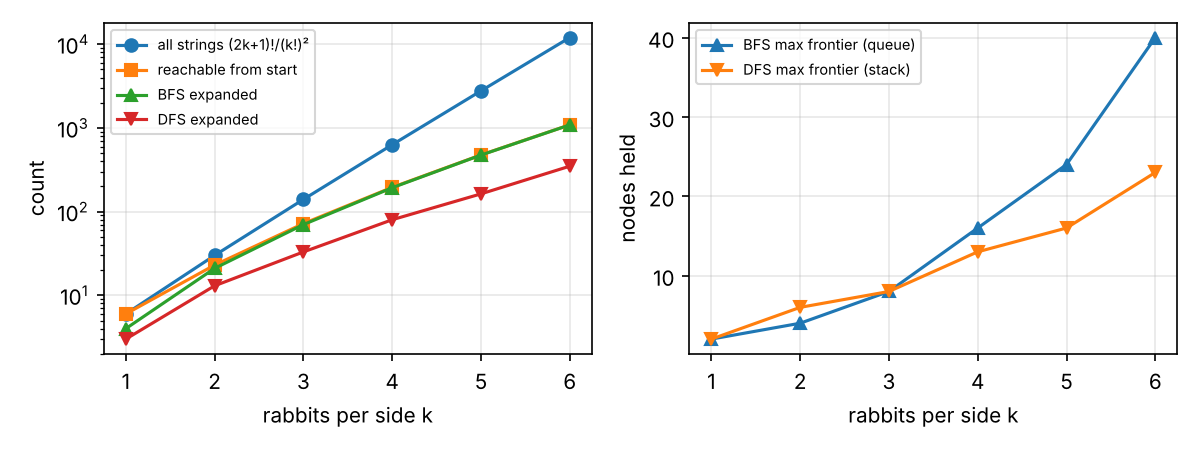
\includegraphics[width=\columnwidth]{rabbit_scaling.png}
\caption{Rabbit Leap with $k$ rabbits per side. Left: the reachable space grows far more
slowly than the syntactic space, and DFS expands about one-third of what BFS expands.
Right: the BFS queue grows faster than the DFS stack.}
\label{fig:rabbitscaling}
\end{figure}

\subsection{Comparison of BFS and DFS}
With branching factor $b$, solution depth $d$ and maximum depth $m$, BFS takes
$O(b^d)$ time and keeps $O(b^d)$ nodes in memory, while DFS takes $O(b^m)$ time but only
$O(bm)$ memory on its stack \cite{aima4}. BFS is complete and optimal for unit costs; DFS
is complete only in finite spaces with repeated-state checking, and is not optimal in
general. In these two puzzles the general caveat about DFS never bites, because all
solutions have the same length; the scaling study in Fig.~\ref{fig:rabbitscaling} (up to
$k=6$: 12\,012 syntactic, 1\,089 reachable states, solution length 48) shows the expected
memory gap, with the BFS queue reaching 40 nodes against 23 for the DFS stack. For larger
graphs with a ``reached'' table, both algorithms are dominated in memory by that table
rather than by the frontier, which is why graph-search DFS loses much of its usual memory
advantage.

%=====================================================================================
\section{Lab 2: Plagiarism Detection as A$^*$ Search}
%=====================================================================================
\subsection{Formulation}
Let document $A$ have sentences $a_1,\dots,a_{n_A}$ and $B$ have $b_1,\dots,b_{n_B}$, after
sentence splitting, lower-casing and punctuation removal. A monotone alignment pairs some
sentences of $A$ with sentences of $B$ in order and leaves the rest unmatched. We search for
the minimum-cost alignment:
\begin{itemize}
\item \textbf{State} $(i,j)$: the first $i$ sentences of $A$ and the first $j$ of $B$ are
aligned. Initial state $(0,0)$, goal $(n_A,n_B)$; there are $(n_A+1)(n_B+1)$ states.
\item \textbf{Actions}: \textsc{Align} $(i,j)\to(i{+}1,j{+}1)$ at cost $d(a_{i+1},b_{j+1})$;
\textsc{SkipA} $(i,j)\to(i{+}1,j)$ and \textsc{SkipB} $(i,j)\to(i,j{+}1)$ at a skip penalty
$p$. Skipping both at once costs $2p \ge d$ and is therefore never useful when $p\ge 0.5$.
\item \textbf{Cost}: the normalised character-level Levenshtein distance \cite{levenshtein1966}
\begin{equation}
d(a,b) = \frac{\operatorname{lev}(a,b)}{\max(|a|,|b|)} \in [0,1],
\end{equation}
computed by the usual dynamic programme with two rows. We use $p=0.5$, so aligning two
unrelated sentences (typical $d\approx0.75$) is still cheaper than skipping both.
\end{itemize}
The path cost is $g(n)$, the sum of the costs along the partial alignment. A$^*$ expands
nodes in order of $f(n)=g(n)+h(n)$ \cite{hart1968}, and with an admissible $h$ the first goal
it pops is a minimum-cost alignment.

\subsection{Heuristics}
Let $r_A = n_A-i$ and $r_B=n_B-j$ be the numbers of sentences still to be aligned. We compare:
\begin{align}
h_0(i,j) &= 0 \quad\text{(uniform-cost search)},\\
h_1(i,j) &= p\,\lvert r_A - r_B\rvert,\\
h_2(i,j) &= \max\bigl(h_1,\; H_A(i,j),\; H_B(i,j)\bigr),
\end{align}
where
\begin{equation}
H_A(i,j) = \sum_{i'>i} \min\Bigl(p,\; \min_{j'>j} \frac{\bigl||a_{i'}|-|b_{j'}|\bigr|}{\max(|a_{i'}|,|b_{j'}|)}\Bigr)
\end{equation}
and $H_B$ is the symmetric sum over $B$'s remaining sentences. $h_1$ is admissible because at
least $\lvert r_A-r_B\rvert$ sentences must still be skipped. $H_A$ is admissible because every
remaining sentence of $A$ must eventually be either skipped (cost $p$) or aligned to some later
sentence of $B$, and the Levenshtein distance is at least the length difference. The suffix
minima are precomputed in $O(n_An_B)$ from sentence lengths alone, so $h_2$ costs no
Levenshtein evaluations. Edit distances are computed lazily and cached, so a better heuristic
also saves distance computations.

\subsection{Detection rule and test cases}
After alignment, a pair with $d\le 0.30$ is flagged as plagiarised and $0.30<d\le0.50$ as
suspicious. All test documents were written for this lab: an eight-sentence paragraph on
stepwells, a lightly paraphrased version of it (synonyms, reordered words), an unrelated
paragraph on filter coffee, an essay that borrows three of the sentences, and a version with
one sentence deleted and one inserted. Results are in Table~\ref{tab:lab2}.

\begin{table}[t]
\centering
\caption{A$^*$ alignment on the test cases ($p=0.5$, 8 sentences per document)}\label{tab:lab2}
\setlength{\tabcolsep}{3.5pt}
\begin{tabular}{@{}lrrrrrr@{}}
\toprule
& & mean & flagged & \multicolumn{3}{c}{nodes expanded} \\
\cmidrule(l){5-7}
Test case & cost & $d$ & of $B$ & $h_0$ & $h_1$ & $h_2$ \\
\midrule
TC1 identical            & 0.000 & 0.000 & 8/8 & 8  & 8  & 8 \\
TC2 slightly modified    & 1.481 & 0.185 & 8/8 & 28 & 16 & 16 \\
TC3 completely different & 5.979 & 0.747 & 0/8 & 80 & 53 & 53 \\
TC4 partial overlap      & 3.981 & 0.498 & 3/8 & 68 & 32 & 32 \\
TC5 deletion + insertion & 1.000 & 0.000 & 7/8 & 28 & 18 & 17 \\
\bottomrule
\end{tabular}
\end{table}

All four required behaviours are reproduced. Identical documents align with zero cost (TC1).
The paraphrase aligns sentence by sentence with distances 0.11--0.27, all below the threshold
(TC2). Unrelated documents align with distances 0.70--0.80 and nothing is flagged (TC3). In
TC4 exactly the three borrowed sentences (positions 3, 5 and 7, two of them lightly edited,
$d=0.000, 0.091, 0.106$) are flagged and the original sentences score 0.73--0.78. In TC5 the
search correctly chooses one \textsc{SkipA} and one \textsc{SkipB} (total cost $2p=1$)
instead of forcing mismatched pairs.

\subsection{Efficiency}
For identical documents every heuristic expands only the diagonal. Elsewhere the heuristics
cut expansions by 34--53\,\%, and the saving persists as documents grow: on synthetic
documents with 10\,\% sentence deletions, 8\,\% insertions and 15\,\% word substitutions,
$h_1$ and $h_2$ expand about half the nodes of $h_0$ (1\,328 vs.\ 2\,655 for 80-sentence
documents) and evaluate only about 21\,\% of the $n_An_B$ sentence pairs
(Fig.~\ref{fig:astar}). The length-based $h_2$ rarely improves on $h_1$, because sentences
of similar length are common, so the length bound is usually much smaller than the true edit
distance. A tighter but still admissible bound (for example a bag-of-characters distance)
would be the natural next step.

\begin{figure}[t]
\centering
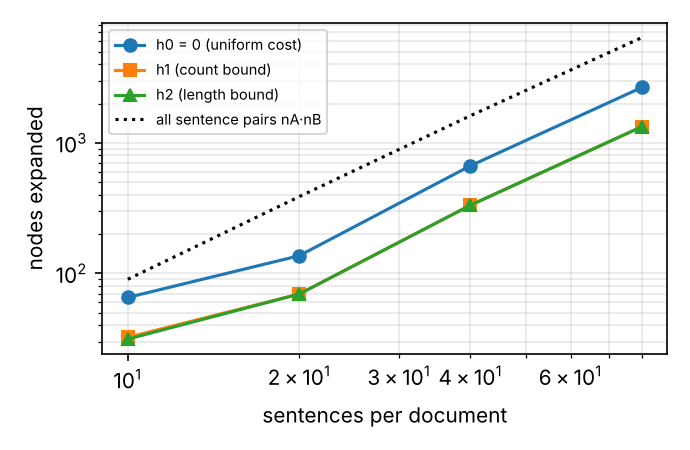
\includegraphics[width=0.85\columnwidth]{astar_scaling.png}
\caption{Nodes expanded by A$^*$ vs.\ document length (mean of three synthetic document pairs).}
\label{fig:astar}
\end{figure}

\emph{Limitations.} The alignment is monotone, so it cannot match sentences that were
reordered; character-level edit distance also underrates heavy paraphrase. Word-level or
embedding-based costs \cite{jurafsky} could be plugged into the same search without
changing the algorithm.

%=====================================================================================
\section{Lab 3: Local Search for Uniform Random 3-SAT}
%=====================================================================================
\subsection{Generating uniform random $k$-SAT instances}
A $k$-SAT formula over $n$ Boolean variables is a conjunction of $m$ clauses, each a
disjunction of $k$ literals. The generator draws each clause independently: $k$
\emph{distinct} variables are sampled uniformly without replacement from $\{x_1,\dots,x_n\}$
and each is negated with probability $1/2$. This is the fixed-clause-length model
\cite{mitchell1992}. For example, $k=3$, $m=5$, $n=4$ gave
\begin{multline*}
(\lnot x_1 \lor x_3 \lor x_4)\land(x_4\lor x_2\lor x_3)\land(x_2\lor\lnot x_3\lor x_1)\\
\land(x_3\lor x_1\lor\lnot x_4)\land(\lnot x_4\lor x_3\lor x_2).
\end{multline*}
The program also writes instances in DIMACS format. Random 3-SAT is hardest near the ratio
$m/n\approx4.26$, where the probability of satisfiability drops from 1 to 0 \cite{mitchell1992}.
We therefore used $n\in\{20,50,100\}$ and $m/n\in\{3.0,4.0,4.3\}$, with 20 instances per
setting (180 in all). Each instance was labelled satisfiable or not with MiniSat through PySAT
\cite{pysat}; the labels are used only to score the local searchers. The satisfiable fraction
fell from 1.00 at $m/n=3$ to 0.75--0.90 at $4.0$ and 0.45--0.55 at $4.3$, as theory predicts.

\subsection{Complete-state formulation and heuristics}
A state is a full assignment $\mathbf{x}\in\{0,1\}^n$, the goal test is that every clause has
a true literal, and neighbours differ in a few variables. Let $t_c(\mathbf{x})$ be the number
of true literals in clause $c$. We maximise one of two heuristics:
\begin{align}
h_1(\mathbf{x}) &= \sum_{c=1}^{m} \mathbb{1}\bigl[t_c(\mathbf{x})\ge1\bigr],\\
h_2(\mathbf{x}) &= h_1(\mathbf{x}) + \frac{1}{m+1}\sum_{c=1}^{m}\mathbb{1}\bigl[t_c(\mathbf{x})\ge2\bigr].
\end{align}
$h_1$ counts satisfied clauses. $h_2$ orders states exactly as $h_1$ does whenever $h_1$
differs (the second term is less than 1), but breaks ties in favour of assignments where more
clauses are satisfied by two or more literals. Such clauses cannot be broken by flipping one
variable, so $h_2$ prefers ``robust'' states and gives the search a gradient on the large
plateaus where $h_1$ is flat.

\subsection{Algorithms}
\emph{Hill-Climbing (HC):} steepest ascent over the $n$ one-flip neighbours, with random tie
breaking; it stops at the first state with no strictly better neighbour.

\emph{Beam Search (BS-$w$, $w\in\{3,4\}$):} starts from $w$ random assignments, generates all
$wn$ one-flip successors, and keeps the $w$ best distinct ones; it stops on a solution or after
$2n$ steps without improving the best score.

\emph{Variable Neighbourhood Descent (VND)} \cite{hansen2001} with three nested neighbourhoods:
$N_1$ flips one variable ($n$ neighbours), $N_2$ flips two variables ($\binom{n}{2}$
neighbours), and $N_3$ flips three variables chosen from those that appear in currently
unsatisfied clauses. VND searches $N_1$; if it cannot improve, it moves to $N_2$, then $N_3$;
after any improvement it returns to $N_1$; it stops when $N_3$ fails.

\subsection{Penetrance}
Following Khemani \cite{khemani}, penetrance measures how directly a search heads to the goal:
\begin{equation}
P = \frac{L}{T},
\end{equation}
where $L$ is the length of the path from the start to the solution (number of moves made) and
$T$ is the total number of nodes generated (here, assignments evaluated). $P=1$ means the search
never evaluated a state off the solution path; failed runs score $P=0$. HC and VND start from
the same random assignment for $h_1$ and $h_2$, so the heuristic comparison is paired.

\begin{table*}[t]
\centering
\caption{Success rate on satisfiable instances (fraction solved) and mean penetrance
$\bar P \times 10^{3}$ for each algorithm and heuristic. Columns are $n$ / $m/n$; the number of
satisfiable instances out of 20 is shown in brackets.}\label{tab:lab3}
\setlength{\tabcolsep}{4pt}
\begin{tabular}{@{}ll*{9}{c}c@{}}
\toprule
& & 20/3.0 & 20/4.0 & 20/4.3 & 50/3.0 & 50/4.0 & 50/4.3 & 100/3.0 & 100/4.0 & 100/4.3 & overall \\
& & [20] & [15] & [10] & [20] & [18] & [11] & [20] & [17] & [9] & [140]\\
\midrule
\multirow{2}{*}{HC}     & $h_1$ & 0.45 & 0.20 & 0.00 & 0.05 & 0.00 & 0.00 & 0.00 & 0.00 & 0.00 & 0.09 \\
                        & $h_2$ & 0.75 & 0.33 & 0.10 & 0.50 & 0.11 & 0.09 & 0.20 & 0.00 & 0.00 & 0.27 \\
\multirow{2}{*}{BS-3}   & $h_1$ & 0.95 & 0.60 & 0.80 & 0.80 & 0.39 & 0.36 & 0.95 & 0.12 & 0.00 & 0.60 \\
                        & $h_2$ & 0.95 & 0.67 & 0.80 & 0.65 & 0.17 & 0.27 & 0.50 & 0.06 & 0.00 & 0.48 \\
\multirow{2}{*}{BS-4}   & $h_1$ & 1.00 & 0.53 & 0.70 & 1.00 & 0.39 & 0.36 & 0.90 & 0.35 & 0.22 & 0.66 \\
                        & $h_2$ & 0.95 & 0.60 & 0.70 & 0.90 & 0.28 & 0.18 & 0.70 & 0.06 & 0.00 & 0.54 \\
\multirow{2}{*}{VND}    & $h_1$ & 0.70 & 0.13 & 0.30 & 0.25 & 0.06 & 0.00 & 0.15 & 0.00 & 0.00 & 0.20 \\
                        & $h_2$ & 0.90 & 0.53 & 0.60 & 0.80 & 0.17 & 0.00 & 0.70 & 0.12 & 0.00 & 0.48 \\
\midrule
\multicolumn{2}{@{}l}{$\bar P\times10^3$:}\\
\multirow{2}{*}{HC}     & $h_1$ & 22.3 & 9.9 & 0.0 & 1.0 & 0.0 & 0.0 & 0.0 & 0.0 & 0.0 & 4.4 \\
                        & $h_2$ & 37.2 & 16.5 & 5.0 & 10.0 & 2.2 & 1.8 & 2.0 & 0.0 & 0.0 & 9.6 \\
\multirow{2}{*}{BS-3}   & $h_1$ & 15.7 & 9.9 & 13.2 & 5.3 & 2.6 & 2.4 & 3.2 & 0.4 & 0.0 & 6.0 \\
                        & $h_2$ & 15.7 & 11.0 & 13.2 & 4.3 & 1.1 & 1.8 & 1.7 & 0.2 & 0.0 & 5.5 \\
\multirow{2}{*}{BS-4}   & $h_1$ & 12.4 & 6.6 & 8.7 & 5.0 & 1.9 & 1.8 & 2.2 & 0.9 & 0.6 & 4.7 \\
                        & $h_2$ & 11.7 & 7.4 & 8.7 & 4.5 & 1.4 & 0.9 & 1.7 & 0.1 & 0.0 & 4.3 \\
\multirow{2}{*}{VND}    & $h_1$ & 25.4 & 4.6 & 8.6 & 1.2 & 0.4 & 0.0 & 0.7 & 0.0 & 0.0 & 5.1 \\
                        & $h_2$ & 40.4 & 20.6 & 20.4 & 12.2 & 1.5 & 0.0 & 4.9 & 0.4 & 0.0 & 12.1 \\
\bottomrule
\end{tabular}
\end{table*}

\begin{figure*}[t]
\centering
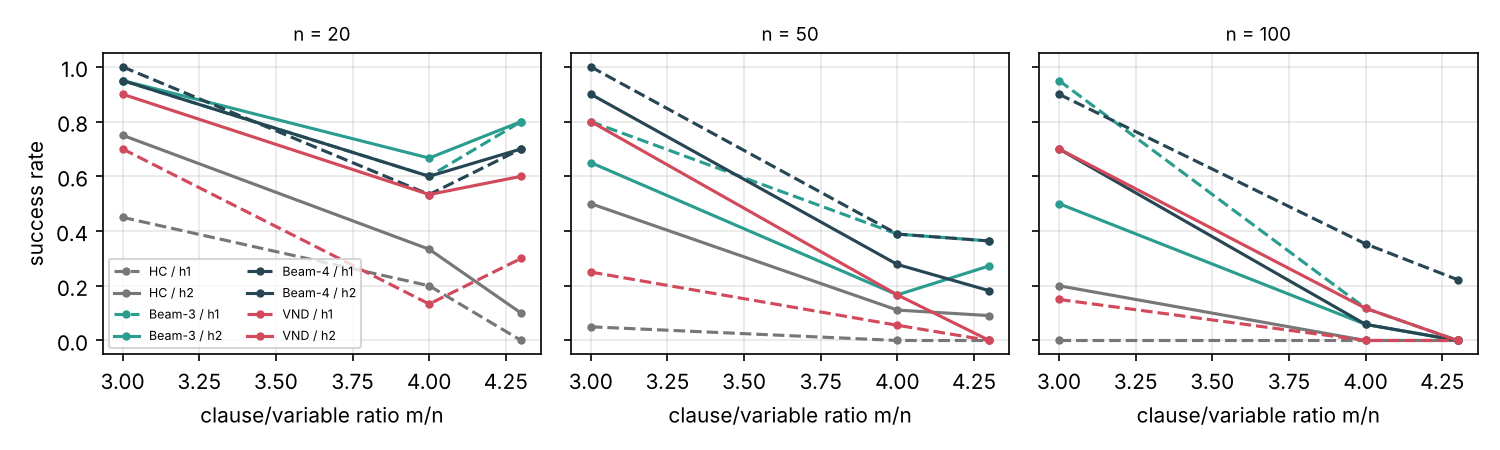
\includegraphics[width=0.49\textwidth]{lab3_success.png}\hfill
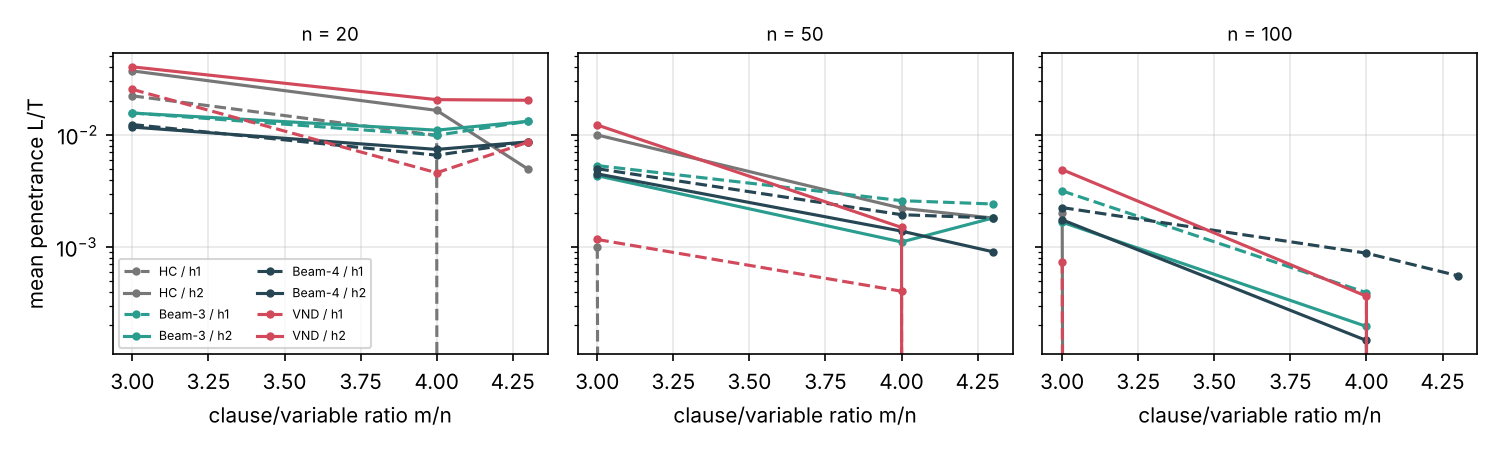
\includegraphics[width=0.49\textwidth]{lab3_penetrance.png}
\caption{Success rate (left) and penetrance on a log scale (right) as the clause ratio $m/n$
approaches the phase transition. Dashed lines: $h_1$; solid lines: $h_2$.}
\label{fig:lab3}
\end{figure*}

\subsection{Results and discussion}
Table~\ref{tab:lab3} and Fig.~\ref{fig:lab3} summarise the 1\,440 runs.
\begin{enumerate}
\item \emph{Difficulty grows with $n$ and with $m/n$.} Every method degrades towards
$m/n=4.3$, and HC solves almost nothing at $n=100$. Under-constrained instances
($m/n=3$) have many solutions, so local optima are rare; near the threshold the landscape is
dominated by plateaus and by local optima that leave only a few clauses unsatisfied (on average
up to 10 for hill-climbing at $n=100$, and 1.5--4 for beam search).
\item \emph{Beam search is the most reliable}, solving 60--66\,\% of satisfiable instances
with $h_1$. It pays for this: it generates $wn$ states per step and, at $n=100$, 35\,000--105\,000
states per run, 15--45 times more than HC. That is why its penetrance is no higher than
VND's despite its higher success rate.
\item \emph{$h_2$ helps single-state searchers.} For HC and VND, which stop as soon as they
see no strict improvement, $h_2$'s tie-breaking turns many plateaus into slopes: success rises
from 0.09 to 0.27 (HC) and 0.20 to 0.48 (VND), and penetrance roughly doubles, with VND+$h_2$
the most efficient method overall ($\bar P = 0.0121$).
\item \emph{$h_2$ hurts beam search slightly.} The beam already escapes plateaus through its
$w$ parallel states and random tie-breaking. With $h_2$ fewer ties exist, so the beam keeps
the $w$ best states, which are often near-duplicates one flip apart, and loses diversity. This
is an example of the general point that a heuristic is good or bad only relative to the
algorithm that uses it.
\item \emph{VND vs.\ HC.} VND's larger neighbourhoods let it leave one-flip local optima
(HC's failure mode), at the price of $\binom{n}{2}$ evaluations whenever it enters $N_2$.
With $h_2$ it more than doubles HC's success at similar cost per solved instance.
\end{enumerate}
None of these methods is complete: a failure does not prove a formula unsatisfiable, which is
why MiniSat was needed to label the instances. Random restarts, sideways moves, or noise in
the style of WalkSAT would raise all success rates; we left them out so that the comparison
isolates the neighbourhood structure and the heuristic.

%=====================================================================================
\section{Lab 4: Simulated Annealing}
%=====================================================================================
\subsection{Simulated annealing in brief}
Simulated annealing (SA) \cite{kirkpatrick1983,delahaye2019} is a local search that sometimes
accepts a worse neighbour. From state $s$ it proposes a random neighbour $s'$ and accepts it
with the Metropolis probability
\begin{equation}
\Pr[\text{accept}] = \min\Bigl(1,\; \exp\Bigl(-\frac{E(s')-E(s)}{T}\Bigr)\Bigr),
\end{equation}
while the temperature $T$ is lowered according to a cooling schedule. At high $T$ the walk is
almost random and crosses energy barriers; as $T\to0$ it becomes a greedy descent. We use
geometric cooling $T_{t+1}=\alpha T_t$, take $T_0$ as the median uphill $\Delta E$ of random
moves (so about 37\,\% of uphill moves are accepted initially), and keep the best state ever
visited.

\subsection{Formulating the jigsaw as a search problem}
The course repository \cite{cs605repo} provides \st{scrambled\_lena.mat}, a $512\times512$
grey-scale image cut into a $4\times4$ grid of $128\times128$ tiles. The file is an Octave text
file whose values are stored column by column, so it is parsed directly rather than with a MAT
reader.
\begin{itemize}
\item \textbf{State}: a permutation $\pi$ of the 16 tiles, $\pi(p)$ = tile at grid position $p$.
Tiles are not rotated in the provided image, so the space has $16!\approx2.09\times10^{13}$
states, far too many for systematic search.
\item \textbf{Moves}: with probability 0.9, swap the tiles at two positions; otherwise make a
\emph{block move}: swap two rows, swap two columns, or cyclically shift all rows or all columns.
\item \textbf{Energy}: the sum of seam dissimilarities over the 24 interior seams,
\begin{equation}
\begin{split}
E(\pi) = &\sum_{(p,q)\in\mathcal{H}} D_{\mathrm{LR}}\bigl(\pi(p),\pi(q)\bigr)\\
       &+ \sum_{(p,q)\in\mathcal{V}} D_{\mathrm{TB}}\bigl(\pi(p),\pi(q)\bigr),
\end{split}
\end{equation}
where $\mathcal{H}$ and $\mathcal{V}$ are the horizontally and vertically adjacent position
pairs. The goal is the minimum-energy arrangement.
\end{itemize}
We compare two seam dissimilarities. Let $\mathbf{u}_1,\mathbf{u}_2$ be the last and second-last
pixel columns of the left tile and $\mathbf{v}_1,\mathbf{v}_2$ the first and second columns of
the right tile.
\begin{enumerate}
\item \emph{Prediction-based L1} \cite{pomeranz2011}: each tile linearly extrapolates its edge
one pixel across the seam,
\begin{equation}
D_{\mathrm{pred}} = \bigl\lVert 2\mathbf{u}_1-\mathbf{u}_2-\mathbf{v}_1\bigr\rVert_1
                  + \bigl\lVert 2\mathbf{v}_1-\mathbf{v}_2-\mathbf{u}_1\bigr\rVert_1 .
\end{equation}
\item \emph{Mahalanobis gradient compatibility (MGC)} \cite{gallagher2012}: the jump across
the seam is compared with the distribution of gradients just inside each tile. With
$\mathbf{g}_u = \mathbf{u}_1-\mathbf{u}_2$ having mean $\mu_u$ and variance $\sigma_u^2$,
\begin{equation}
\begin{split}
D_{\mathrm{MGC}} = &\sum_{r}\frac{\bigl(v_{1r}-u_{1r}-\mu_u\bigr)^2}{\sigma_u^2+\epsilon}\\
                 &+ \sum_{r}\frac{\bigl(u_{1r}-v_{1r}-\mu_v\bigr)^2}{\sigma_v^2+\epsilon},
\end{split}
\end{equation}
with $\epsilon=1$. A seam that crosses a genuine strong edge (such as the boundary of the
mirror frame in Lena) is penalised less if both tiles already contain strong gradients.
\end{enumerate}

\subsection{Results}
Each configuration was run from 10 random permutations with $\alpha=0.9995$ for 60\,000
iterations. Both energies have the same global optimum, and it is the true image
(Fig.~\ref{fig:jigsaw}): $E_{\mathrm{pred}}$ drops from 338\,536 for the scrambled input to
52\,013, and $E_{\mathrm{MGC}}$ from $3.32\times10^6$ to 6\,896. All 24 seams of the two
solutions agree. Table~\ref{tab:jigsaw} shows how often each variant reaches that optimum.

\begin{figure}[t]
\centering
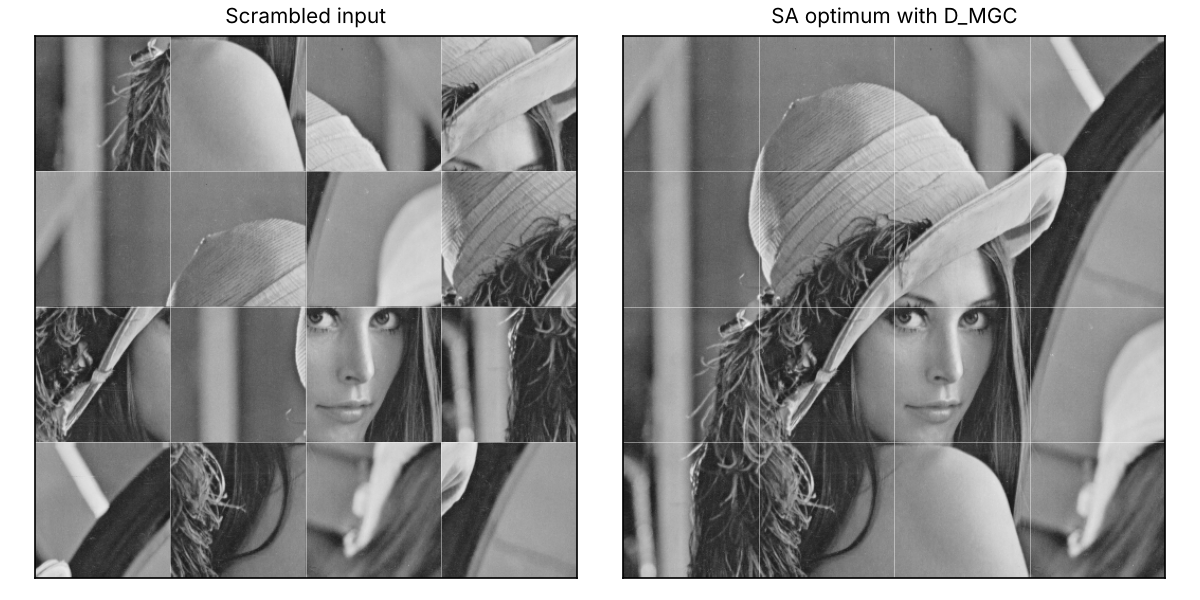
\includegraphics[width=\columnwidth]{jigsaw_before_after.png}
\caption{Left: the scrambled input. Right: the SA solution (all 10 MGC restarts reach it).}
\label{fig:jigsaw}
\end{figure}

\begin{table}[t]
\centering
\caption{Restarts (out of 10) that reach the global optimum}\label{tab:jigsaw}
\begin{tabular}{@{}lcc@{}}
\toprule
Method & $D_{\mathrm{pred}}$ & $D_{\mathrm{MGC}}$ \\
\midrule
SA, swaps + block moves       & 5 & 10 \\
SA, swaps only                & 1 & 10 \\
Greedy descent ($T\approx0$), all moves & 0 & 6 \\
\bottomrule
\end{tabular}
\end{table}

Three lessons follow.
\begin{enumerate}
\item \emph{Annealing beats greedy descent.} With the same moves and iteration budget,
descent at $T\approx0$ never solved the puzzle with $D_{\mathrm{pred}}$; SA solved it in half
the restarts (Fig.~\ref{fig:jigsawtrace}).
\item \emph{The move set shapes the landscape.} The most frequent wrong answers with swap-only
moves (energies 81\,781--83\,420) are the correct image cyclically shifted by one column or row.
Undoing such a shift needs several coordinated swaps, each of which breaks good seams, so SA has
to climb a high barrier. A single ``shift all columns'' move removes that barrier and raised
success from 1/10 to 5/10. In general, adding a move that connects two deep basins can matter
more than tuning the cooling schedule.
\item \emph{The energy shapes the landscape too.} MGC separates the true seams from false ones
by a much wider margin, so the correct basin is far deeper; with MGC even greedy descent
succeeds 6/10 times and SA succeeds every time.
\end{enumerate}

\begin{figure}[t]
\centering
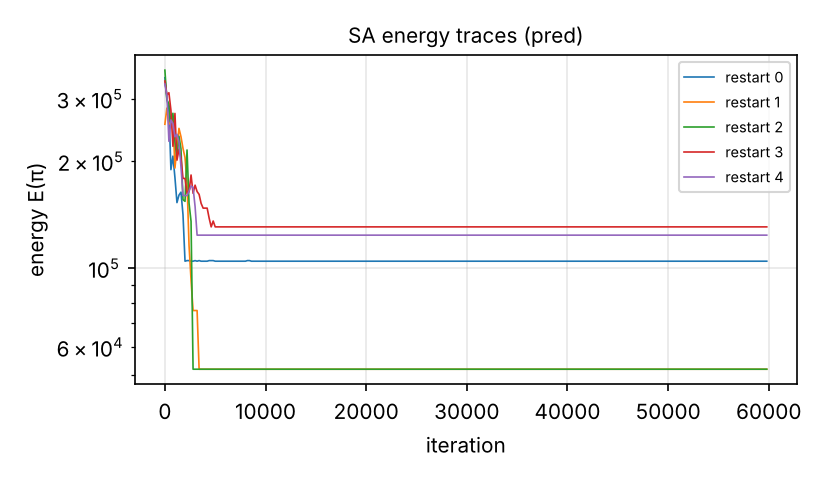
\includegraphics[width=\columnwidth]{jigsaw_energy_trace_pred.png}
\caption{SA energy traces with $D_{\mathrm{pred}}$ (log scale). Runs that end at higher energy
are trapped in shifted arrangements.}
\label{fig:jigsawtrace}
\end{figure}

\subsection{In-lab problem: a tour of Rajasthan}
We chose 20 places (Jaipur, Ajmer, Pushkar, Jodhpur, Jaisalmer, Bikaner, Udaipur, Mount Abu,
Chittorgarh, Kumbhalgarh, Ranakpur, Nathdwara, Bundi, Kota, Sawai Madhopur, Bharatpur, Alwar,
Mandawa, Abhaneri, Osian), used their approximate latitude and longitude, and took the travel
cost proportional to the great-circle (haversine) distance, as the problem allows. SA used 2-opt
moves (reverse a segment of the tour), whose cost change is computed in $O(1)$:
\begin{equation}
\Delta L = d(t_{i-1},t_j)+d(t_i,t_{j+1})-d(t_{i-1},t_i)-d(t_j,t_{j+1}).
\end{equation}
Because 20 cities are within reach of the exact Held--Karp dynamic programme
\cite{heldkarp1962} ($O(2^{n}n^{2})$), we could check the SA answer: 9 of 10 SA restarts found
the optimal 2\,149\,km tour (the tenth found 2\,153.5\,km). The tour is Jaipur $\to$ Ajmer
$\to$ Pushkar $\to$ Mandawa $\to$ Bikaner $\to$ Jaisalmer $\to$ Osian $\to$ Jodhpur $\to$
Kumbhalgarh $\to$ Ranakpur $\to$ Mount Abu $\to$ Udaipur $\to$ Nathdwara $\to$ Chittorgarh
$\to$ Bundi $\to$ Kota $\to$ Sawai Madhopur $\to$ Bharatpur $\to$ Alwar $\to$ Abhaneri $\to$
Jaipur (Fig.~\ref{fig:tsp}). Real road distances are longer than great-circle distances, but
the ranking of tours is usually similar. The VLSI benchmark files could not be downloaded in
our environment; the code includes a TSPLIB reader so the same SA runs on them unchanged.

\begin{figure}[t]
\centering
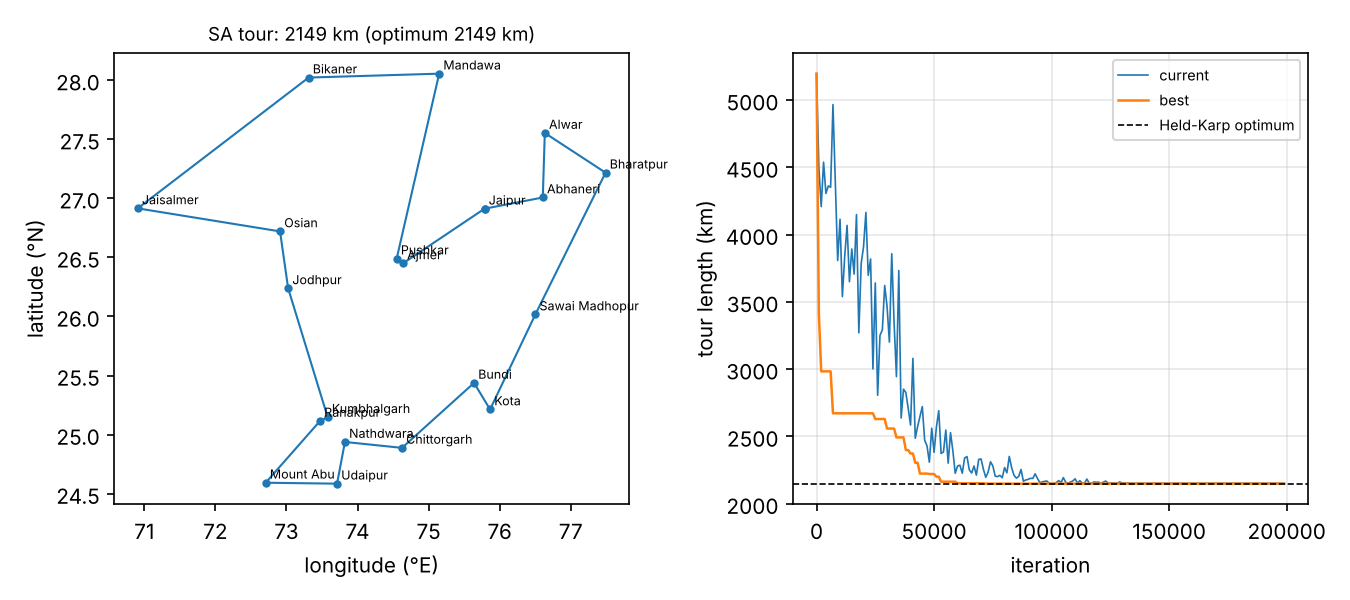
\includegraphics[width=\columnwidth]{tsp_rajasthan.png}
\caption{Left: optimal tour found by SA. Right: current and best tour length during the best
run, with the Held--Karp optimum.}
\label{fig:tsp}
\end{figure}

\subsection{Challenge problem: a melody in Raag Bhairav}
A melody is a sequence of 32 swaras (four 8-beat phrases) drawn from the Bhairav scale:
S, komal r, G, m, P, komal d, N, with mandra P., d., N.\ and taar S$'$. Because only these
swaras can be represented, no foreign note can ever appear. The energy encodes the raag's
grammar as described in \cite{bhairavref}: aaroh S r G m P d N S$'$ and avroh S$'$ N d P m G
r S, pakad ``G m d d P, G m r r S'', vadi d and samvadi r, and nyaas on S, r, m, P, d. It is the
sum of penalties for (i) leaps of more than five semitones other than S--P, (ii) moves that skip
more than one swara of the scale, (iii) phrase endings away from nyaas swaras and a final note
other than S, (iv) d and r appearing less than 18\,\% and 14\,\% of the time, (v) missing
characteristic phrases, weighted by importance, and (vi) the same swara three times in a row.
SA moves change one swara, move one swara a step up or down, or copy a 3--5-note window
elsewhere, which encourages the motif repetition typical of a bandish.

The best of eight runs reached zero energy:
\begin{center}\small
\texttt{| N. S r S r G m d | d P N d P m G r |}\\
\texttt{| S G r m d d N S' | N d P G m r r S |}
\end{center}
It contains both halves of the pakad (``G m d d P'' across the first bar line and
``G m r r S'' at the end), the descent ``S$'$ N d P'', the cadence ``m G r S'' and the
opening ``N.\ S r S'', and ends on Sa. The script also writes a WAV rendering with a Sa--Pa
drone and a slight oscillation on komal r and d to imitate andolan. The energy captures the
grammar of the raag but not its aesthetics: slow andolan, meend between notes and the timing
of phrases matter as much in Bhairav as the swaras themselves, and an evaluation by a trained
listener would be the real test.

%=====================================================================================
\section{Conclusion}
%=====================================================================================
The same few ideas recur across all four labs. A compact formulation matters more than the
search algorithm: interchangeable people turn the river crossing into 16 reachable states, and
the $(i,j)$ prefix state turns plagiarism detection into a grid shortest-path problem. Problem
structure explains algorithm behaviour, as in the counting argument that makes DFS optimal for
Rabbit Leap. A heuristic's value depends on the algorithm using it, as $h_2$ helping
hill-climbing but hurting beam search shows. And for randomised search, the energy and the move
set, not just the temperature schedule, decide which basins the search can reach.

\bibliographystyle{IEEEtran}
\bibliography{refs}

\end{document}
